\documentclass[11pt,a4paper,oneside]{article}
\usepackage[UTF8,adobefonts]{ctex}

\usepackage{wrapfig}
\usepackage{indentfirst}
\usepackage{amsmath}
\usepackage{float}
\usepackage{ulem}

\usepackage[top=1in,bottom=1in,left=1.25in,right=1.25in]{geometry}

\usepackage{color}
\usepackage{xcolor}

\usepackage{multirow}
\usepackage{amssymb}
\usepackage{graphicx}

\usepackage{diagbox}
\usepackage{slashbox}
\begin{document}
\section*{五、实验数据处理}

\section*{实验1.测定冰的熔解热}

\subsection*{(1)原始数据记录}
\textbf{初始每隔60s记录表}
\begin{tabular}{|c|c|c|}
\hline 
时间/s & 阻值/k$\Omega$ & 温度/$^{\circ}C$
\\
\hline

0 & 1.1488 & 38.29
\\
\hline

60 & 1.1484 & 38.19
\\
\hline

120 & 1.1483 & 38.16
\\
\hline

180 & 1.1482 & 38.14
\\
\hline

240 & 1.1481 & 38.11
\\
\hline

300 & 1.1480 & 38.09
\\
\hline

360 & 1.1479 & 38.06
\\
\hline

420 & 1.1478 & 38.03
\\
\hline

\end{tabular} 

\vspace{1.5cm}

\textbf{每隔15s记录表}
\begin{tabular}{|c|c|c|}
\hline 
时间/s & 阻值/k$\Omega$ & 温度/$^{\circ}C$
\\
\hline

480 & 1.1450 & 37.31
\\
\hline

495 & 1.1449 & 37.28
\\
\hline

510 & 1.1448 & 37.26
\\
\hline

\end{tabular} 

\vspace{1.5cm}
\textbf{最后每隔60s记录表}
\begin{tabular}{|c|c|c|}
\hline 
时间/s & 阻值/k$\Omega$ & 温度/$^{\circ}C$
\\
\hline

525 & 1.1470 & 37.83
\\
\hline

585 & 1.1471 & 37.85
\\
\hline

645 & 1.1472 & 37.88
\\
\hline

\end{tabular}

\begin{figure}[H]
 \centering
  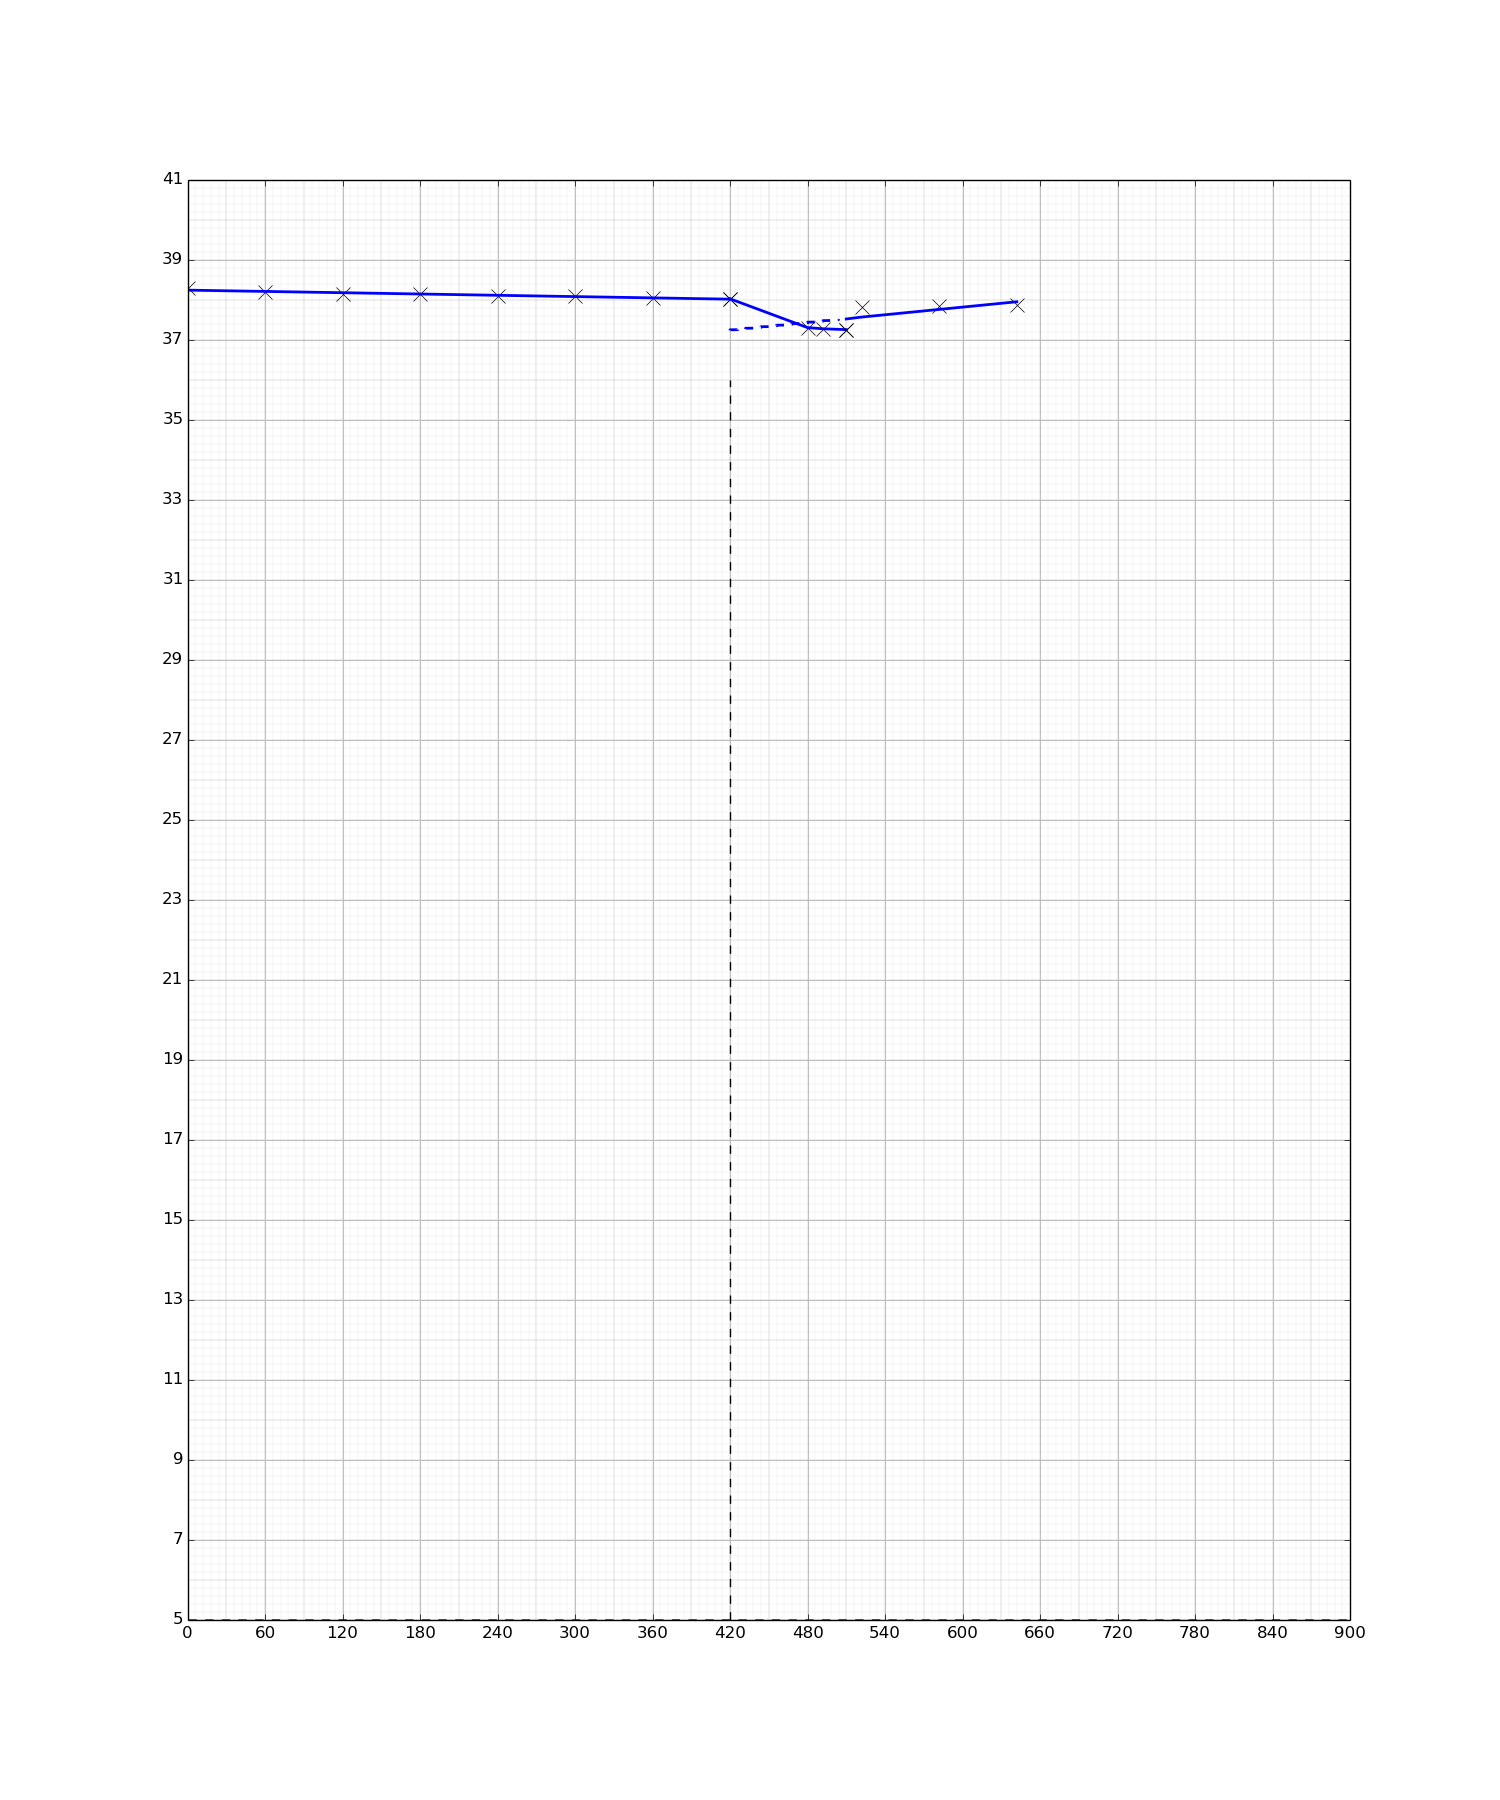
\includegraphics[width=13cm]{/var/www/buaaphylab/public/pdf_tmp/df7f6a69678d0de757793419305b3b2e.png}
\end{figure}

图中竖线的横坐标为421。
\end{document}